\documentclass[12pt, notitlepage]{article}
\usepackage[margin=1in, top=0.5in]{geometry}
\usepackage[utf8x]{inputenc}
\usepackage{gensymb}
\usepackage{array}
\usepackage{amssymb}
\usepackage{amsmath}
\usepackage{graphicx}
\usepackage{tabularx}
\usepackage{pbox}
\usepackage[makeroom]{cancel}
\usepackage{float}
\usepackage{caption}
\usepackage{newfloat}
\DeclareFloatingEnvironment[name={Gráfico}]{graph}
\newcommand\numberthis{\addtocounter{equation}{1}\tag{\theequation}}

\title{Título}

\date{\today}
\renewcommand\refname{Referencias}
\renewcommand\tablename{Tabla}
\renewcommand\figurename{Figura}
\newcommand{\norm}[1]{\left\lVert#1\right\rVert}

\geometry{letterpaper}

\begin{document}
\thispagestyle{empty}
\setlength{\unitlength}{1 cm} %Especificar unidad de trabajo
\begin{picture}(18,4)
\put(0,0){
\includegraphics[scale=0.38]{UTFSM_logo.png}}
\put(11.5,0){
\includegraphics[scale=0.2]{mecusm.jpg}}
\end{picture}
\\
\\
\begin{center}
{\LARGE {Universidad Técnica Federico Santa María}}\\[0.5cm]
{\Large Departamento de Ingeniería Mecánica}\\[2cm]
%{\Large Redes}\\[2.3cm]
{\Huge \textbf{Tarea 4:}}\\[0.2cm]
{\Huge \textbf{``Método de Runge-Kutta aplicado a una E.D.O. de 2\degree orden."}}\\[0.2cm]
{\large IPM-458 - Computación Científica.}\\[3cm]
{\large Alumno: Nicolás Espinoza M.}\\[3cm]
Profesor: Franco Perazzo M.\\
Ayudante: Luis Fuenzalida L.\\[3cm]
Valparaíso - Junio 23, 2017
\end{center}
\newpage
\tableofcontents
\newpage

\section{Introducción al Problema.}
En ingeniería y ciencias se utilizan innumerables ecuaciones que modelan el mundo real, y los acontecimientos que allí ocurren, para poder entenderlos y ser capaces de desenvolverse mejor. Sin embargo, encontrar una solución analítica para dichas ecuaciones no siempre resulta posible, debido a la gran complejidad que presentan. En estos casos se emplean métodos de resolución numérica que aproximan las soluciones con un cierto grado de error. En este informe se revisa el caso de una interfaz de fluido-gas, en particular una burbuja. La ecuación que se debe aproximar es la siguiente:

\begin{equation}
\frac{d^2A}{d\tau^2} + 3\frac{dA}{d\tau} + \left[2 - \frac{\alpha}{\beta e^\tau}\left(1 - \frac{1}{\beta^2e^{2\tau}}\right)\right]A = 0
\end{equation}

Las expresiones que definen $\alpha \text{ y } \beta$ se entregan más adelante en el informe.
La ecuación no tiene una resolución directa simple, por lo que se procede a desarrollar un método de Runge-Kutta de cuarto orden para aproximar las soluciones.

\section{Método de Runge-Kutta}
Lo que se hace en el método de Runge-Kutta es intentar aproximar la función en $n$ puntos, haciendo un promedio ponderado de la variación de la variable dependiente contra el tiempo. Esto se logra en este problema con un sistema de ecuaciones de $2\text{x}2$

\begin{gather}
\psi = \frac{dA}{d\tau}\\
\frac{d\psi}{d\tau} = \frac{d^2A}{d\tau^2}
\end{gather}

Sabemos que la Ecuación (1) se puede escribir también despejando $d^2A/d\tau^2$
\begin{equation*}
\frac{d^2A}{d\tau^2} = - 3\frac{dA}{d\tau} - \left[2 - \frac{\alpha}{\beta e^\tau}\left(1 - \frac{1}{\beta^2e^{2\tau}}\right)\right]A
\end{equation*}

por lo que tenemos una expresión para la Ecuación (3) que nos permita resolver el sistema si tenemos condiciones iniciales.\\\\
El método de Runge-Kutta de cuarto orden nos significa una mayor precisión, equivalente a truncar una serie de Taylor en el elemento de $3^{er}$ orden; el orden del error es $O(h^4)$. Para trabajar con este método, hay que aplicar un método de Euler, pero se mejora la precisión al trabajar con pasos intermedios a los pasos $t_i, t_{i+1}$. El argumento de una aproximación con el método de Euler sale de una función $y'_i = f(t_i,y_i)$, omitiendo condiciones iniciales. Esta función viene de una expansión de Taylor truncada en el término de primer orden, quedando $y_{i+1} = y_i + h\cdot f(t_i, y_i)$.\\
Sin embargo, para el método de Runge-Kutta se tienen aproximaciones a medio paso también:

\begin{gather*}
y_{i+1} = y_i + \frac{1}{6}(k1 + 2(k2 + k3) + k4)\cdot h \numberthis\\
k1 = h\cdot f(t,y_i) \qquad k2 = h\cdot f(t+h/2, y_i + k1/2)\\
k3 = h\cdot f(t + h/2, y_i + k2/2) \qquad k4 = h\cdot f(t + h, y_i + k3)
\end{gather*}

Con esto se puede interpolar el valor de la función entre los puntos dados por el paso de tiempo. La ventaja es la facilidad de implementación del método en computadores, pues es aproximadamente de la misma complejidad (en términos informáticos) que una aproximación por el método de Euler explícito.

\section{Presentación de resultados}
A partir del método de Runge-Kutta aplicado a la Ecuación (1) se obtienen las curvas de la amplitud de oscilación de la perturbación en una interfaz gas-fluido (burbuja) en función del tiempo para distintos valores de los parámetros $\alpha \text{ y } \beta$

\begin{gather*}
\alpha = \frac{2\pi R}{\lambda_c}\qquad\qquad\beta = \frac{\lambda_0}{\lambda_c}\qquad\qquad \lambda_c = 2\pi\sqrt{\frac{\sigma}{\rho g}}
\end{gather*}

Los valores que se usaron son $\alpha = 50\text{, }65 \text{ y } 80$, y en cada gráfico se grafican todos los valores de beta; estos son $\beta = 0.33, 0.50, 0.67, 0.91, 1.00, 1.33 \text{ y } 2.00$. También se presenta la curva que se toma como referencia, al menos cualitativa, de la publicación en la revista \textit{Journal of Fluid Mechanics}[1]. Las gráficas siguientes tienen como variable independiente no el tiempo adimensional $\tau$, sino que $\hat{\tau} = \tau - ln(\beta)$ para lograr que todas estén centradas. Los valores de entrada para el programa son $h = 0.05$, $y_0 = 0$, $\left.\frac{dA}{d\tau}\right|_0 = 1$.

\begin{figure}[H]
\centering
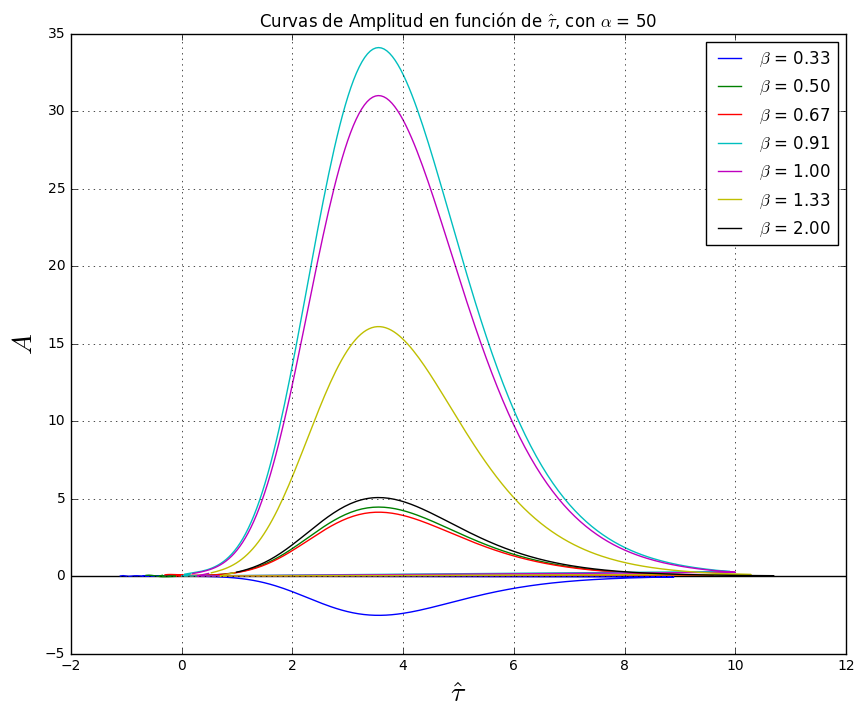
\includegraphics[scale = 0.6]{alfa50.png}
\caption{Gráfico para la amplitud en función de $\hat{\tau}$ para $\alpha = 50$}
\end{figure}

\begin{figure}[H]
\centering
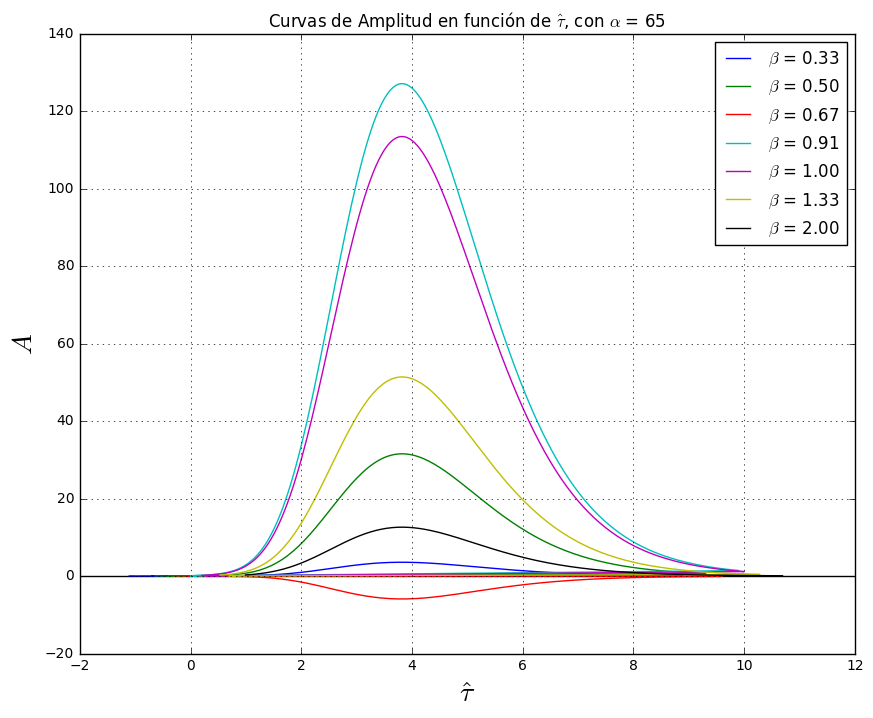
\includegraphics[scale = 0.55]{alfa65.png}
\caption{Gráfico para la amplitud en función de $\hat{\tau}$ para $\alpha = 65$}
\end{figure}

\begin{figure}[H]
\centering
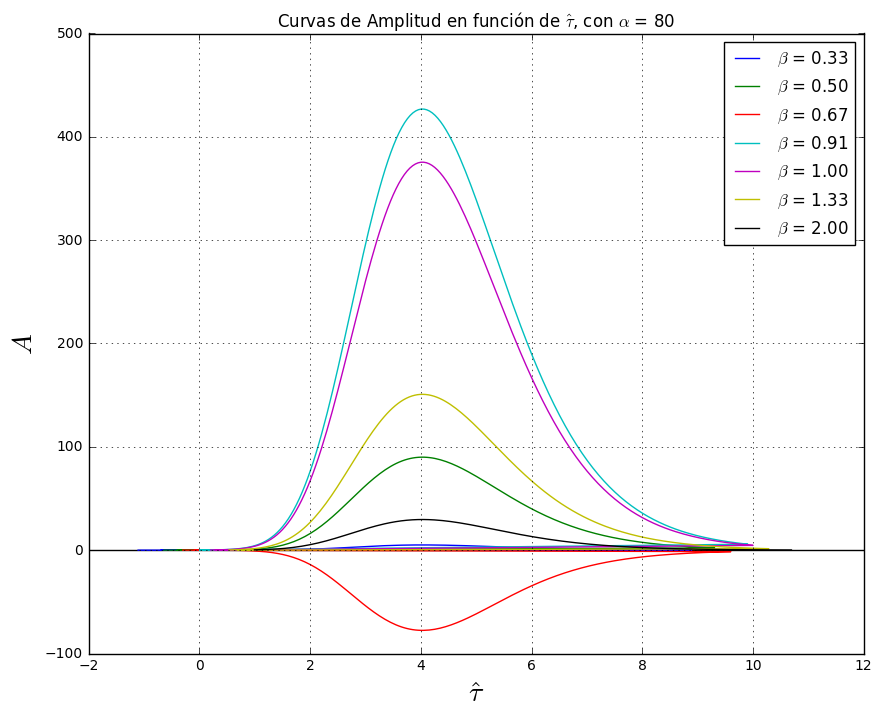
\includegraphics[scale = 0.55]{alfa80.png}
\caption{Gráfico para la amplitud en función de $\hat{\tau}$ para $\alpha = 80$}
\end{figure}

\begin{figure}
\centering
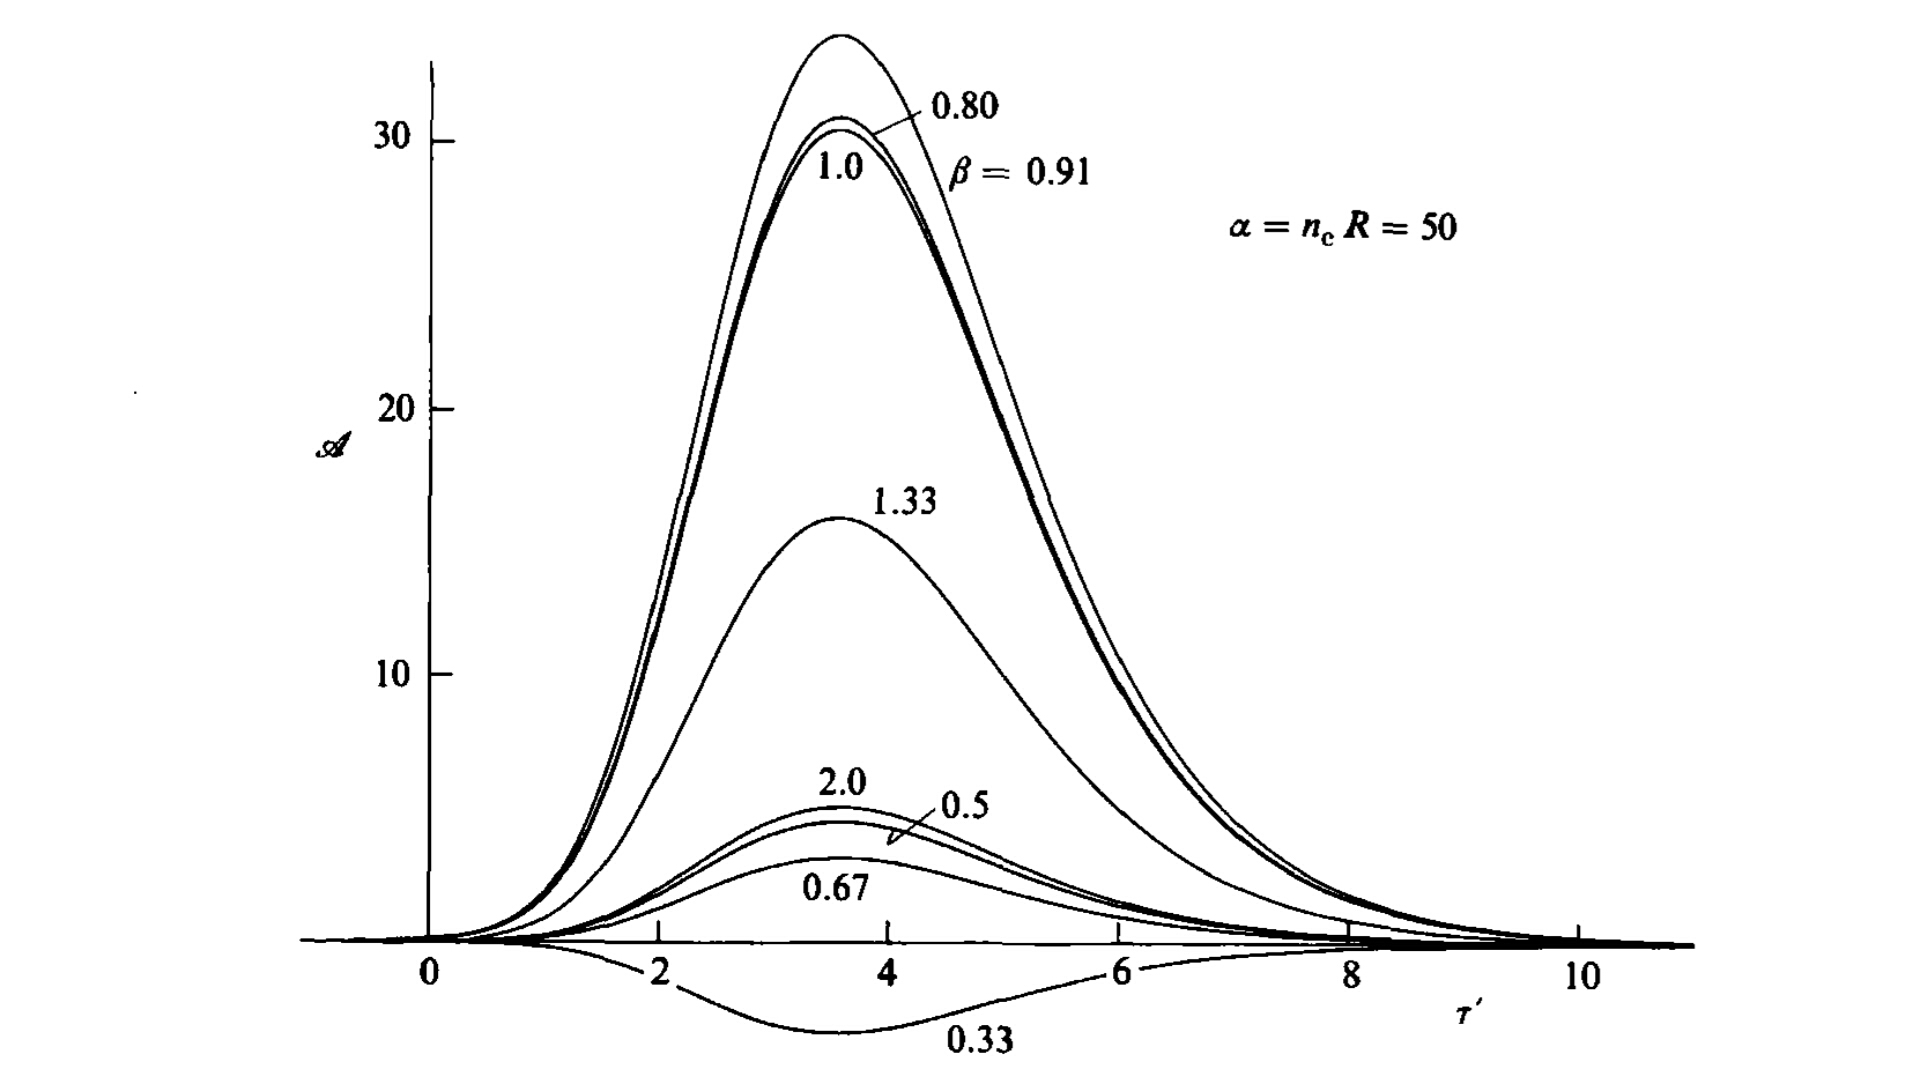
\includegraphics[scale=0.25]{asd1.jpg}
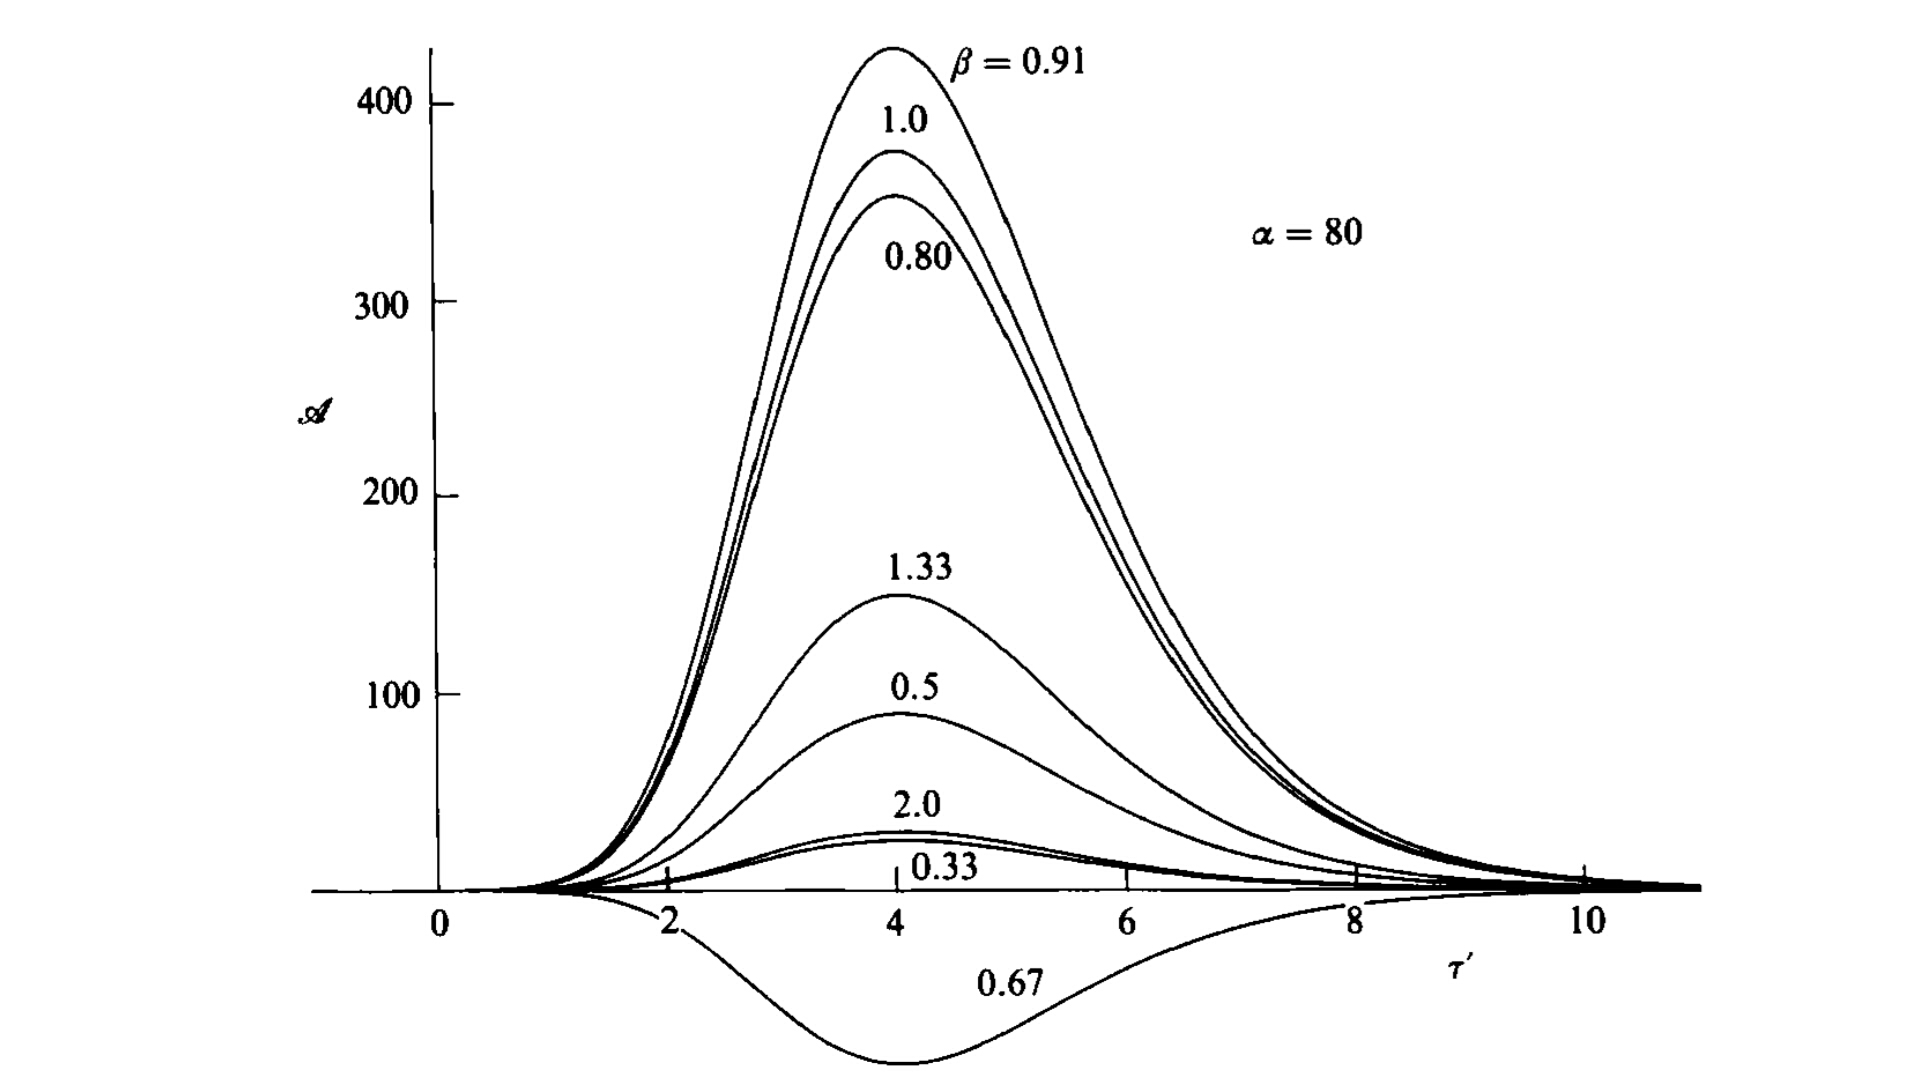
\includegraphics[scale=0.25]{asd2.jpg}
\caption{Gráfico para la amplitud en función del tiempo usados como referencia de la revista \textit{Journal of Fluid Mechanics} [1]. El superior es con $\alpha = 50$, el inferior con $\alpha = 80$}
\end{figure}

\section{Análisis y conclusiones}

En los gráficos se puede observar cómo varía la amplitud de la perturbación sobre la interfaz a medida que se varían los parámetros. El parecido entre el gráfico de la Figura 1 y el gráfico superior de la Figura 4, y la Figura 2 y el gráfico inferior de la Figura 4, hace evidente que el método de Runge-Kutta de orden 4 es muy efectivo para aproximar resultados de funciones a través de métodos numéricos que sean computacionalmente eficientes y a la vez simples.\\\\
Además, es posible guardar los valores ya sea en un arreglo como en un archivo, permitiendo elegir cómo administrar el uso de memoria dependiendo de los requisitos y la complejidad del problema. Por último, como RK4 es un método con error de orden 4, para este ejercicio ese valor es del orden de $(5\cdot 10^{-2})^4 \approx 10^{-5}$.\\\\
En resumen, es preferente el uso de un método RK4 para la resolución de sistemas de EDOs si se conocen los valores iniciales de las variables dependiente e independiente.

\begin{thebibliography}{1}
\item{G. K. Batchelor (1987). The stability of a large gas bubble rising through liquid. Journal of Fluid Mechanics, 184, pp 399-422 doi:10.1017/S0022112087002945}
\end{thebibliography}

\end{document}